\chapter{Experimental Methodology}
\label{methodology}

\section{Anechoic Chamber}
All experiments were conducted at the GDTL within the Aerospace Research Center at the Ohio State University. 
Compressed, dried, and filtered air is supplied to the facility from two cylindrical storage tanks with a total capacity of 43 m$^{3}$ and maximum storage pressure of 16 MPa.
The air may be routed through a storage heater (not used in this study), which allows the jet to operate with a stagnation temperature up to 500 C, before expanding through a nozzle and exhausting horizontally into an anechoic chamber. 
Opposite the nozzle, a collector accumulates the jet and entrained air and exhausts to the outdoors. 
A schematic of the anechoic chamber can be seen in [INSERT FIGURE]. 
The dimensions of the chamber are 6.20 m wide by 5.59 m long and 3.36 m tall, with internal wedge-tip to wedge-tip dimensions of 5.14 m by 4.48 m and 2.53 m, respectively. 
The design of the chamber produces a cutoff frequency of 160 Hz, below the frequencies of interest for this study. 
A more detailed description of the GDTL anechoic chamber properties and validation has been given by [Hahn?].
\begin{figure}
	\centering
	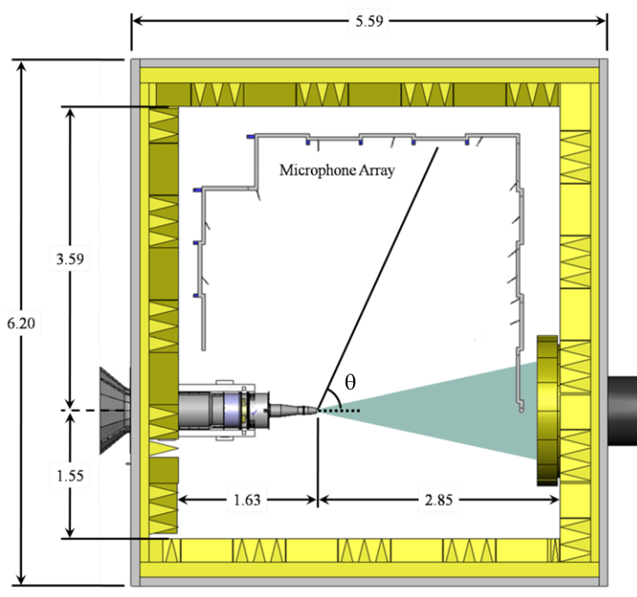
\includegraphics{Figures/Chamber_Schematic.png}
	\caption{???} \label{fig:chamber}
\end{figure}

For this study a converging, axisymmetric nozzle with exit diameter D of 25.4 mm was used. 
The internal contour of the nozzle was designed using a fifth order polynomial. 
The nozzle utilized a thick-lipped design in order to simplify the mounts for the LAFPA extension, which housed the eight actuators used in this study. 
For the experiments reported in this paper, the jet was operated at a Mach number ($M_j$) of 0.90, and with a total temperature ratio of approximately unity. 
The Reynolds number based on the jet exit diameter was $6.2 \times〖10〗^5$; previous investigations using hot-wire anemometry have indicated that the initial shear layer is turbulent for this operating condition with momentum thickness ~0.09 mm and boundary layer thickness ~1 mm [Kearney?].

\section{Data Acquisition}
\subsection{Near- and Far-field Pressure}
Near-field and far-field pressure measurements were acquired simultaneously, using Brüel \& Kjær ¼ inch 4939 microphones. 
The signal from each microphone is band-pass filtered from 20 Hz to 100 kHz using a Brüel \& Kjær Nexus 2690 conditioning amplifier, and recorded using National Instruments PXI-6133 A/D boards and LabVIEW software. 
The microphones are calibrated using a Brüel \& Kjaer 114 dB, 1 kHz sine wave generator (model \# ???). 
The frequency response of the microphones is flat up to roughly 80 kHz, with the protective grid covers removed. 

\subsection{Particle Image Velocimetry}

\section{Localized Arc-Filament Plasma Actuators}